\documentclass[final,hyperref={pdfpagelabels=false}, professionalmath, mathserif, 11pt]{beamer}
\usepackage{grffile}
\mode<presentation>{\usetheme{BGC_retreat}}
\usepackage[english]{babel}
\usepackage[utf8]{inputenc}
\usepackage{graphicx}
\usepackage[round]{natbib}

 
\def\mytitle{SoilR and a General SOM Decompositon Model }
%\def\mysubtitle{Application to Stability}
\def\myauthor{Markus Müller \quad Carlos Sierra }
\def\myfooterleft{
    \begin{minipage}[T]{.95\textwidth}

\begin{thebibliography}{15}
%\providecommand{\natexlab}[1]{#1}
%\providecommand{\url}[1]{\texttt{#1}}
%\expandafter\ifx\csname urlstyle\endcsname\relax
%  \providecommand{\doi}[1]{doi: #1}\else
%  \providecommand{\doi}{doi: \begingroup \urlstyle{rm}\Url}\fi


\bibitem[Sierra et~al.(2012)Sierra, M\"uller, and Trumbore]{SierraGMD}
C.~A. Sierra, M.~M\"uller, and S.~E. Trumbore.
\newblock Models of soil organic matter decomposition: the {SoilR} package,
  version 1.0.
\newblock \emph{Geosci. Model Dev.}, 5\penalty0 (4):\penalty0 1045--1060, 2012.
\newblock GMD.

\bibitem[Sierra et~al.(2014)Sierra, M\"uller, and Trumbore]{SierraGMD14}
C.~A. Sierra, M.~M\"uller, and S.~E. Trumbore.
\newblock Modeling radiocarbon dynamics in soils: {SoilR} , version 1.1.
\newblock \emph{Geosci. Model Dev.}, 7\penalty0 (7):\penalty0 1919--1931, 2014.
\newblock GMD.

\end{thebibliography}
     \end{minipage}
}
\def\myfooterright{
    \begin{minipage}[T]{.95\textwidth}
	\begin{minipage}[c]{5cm}
	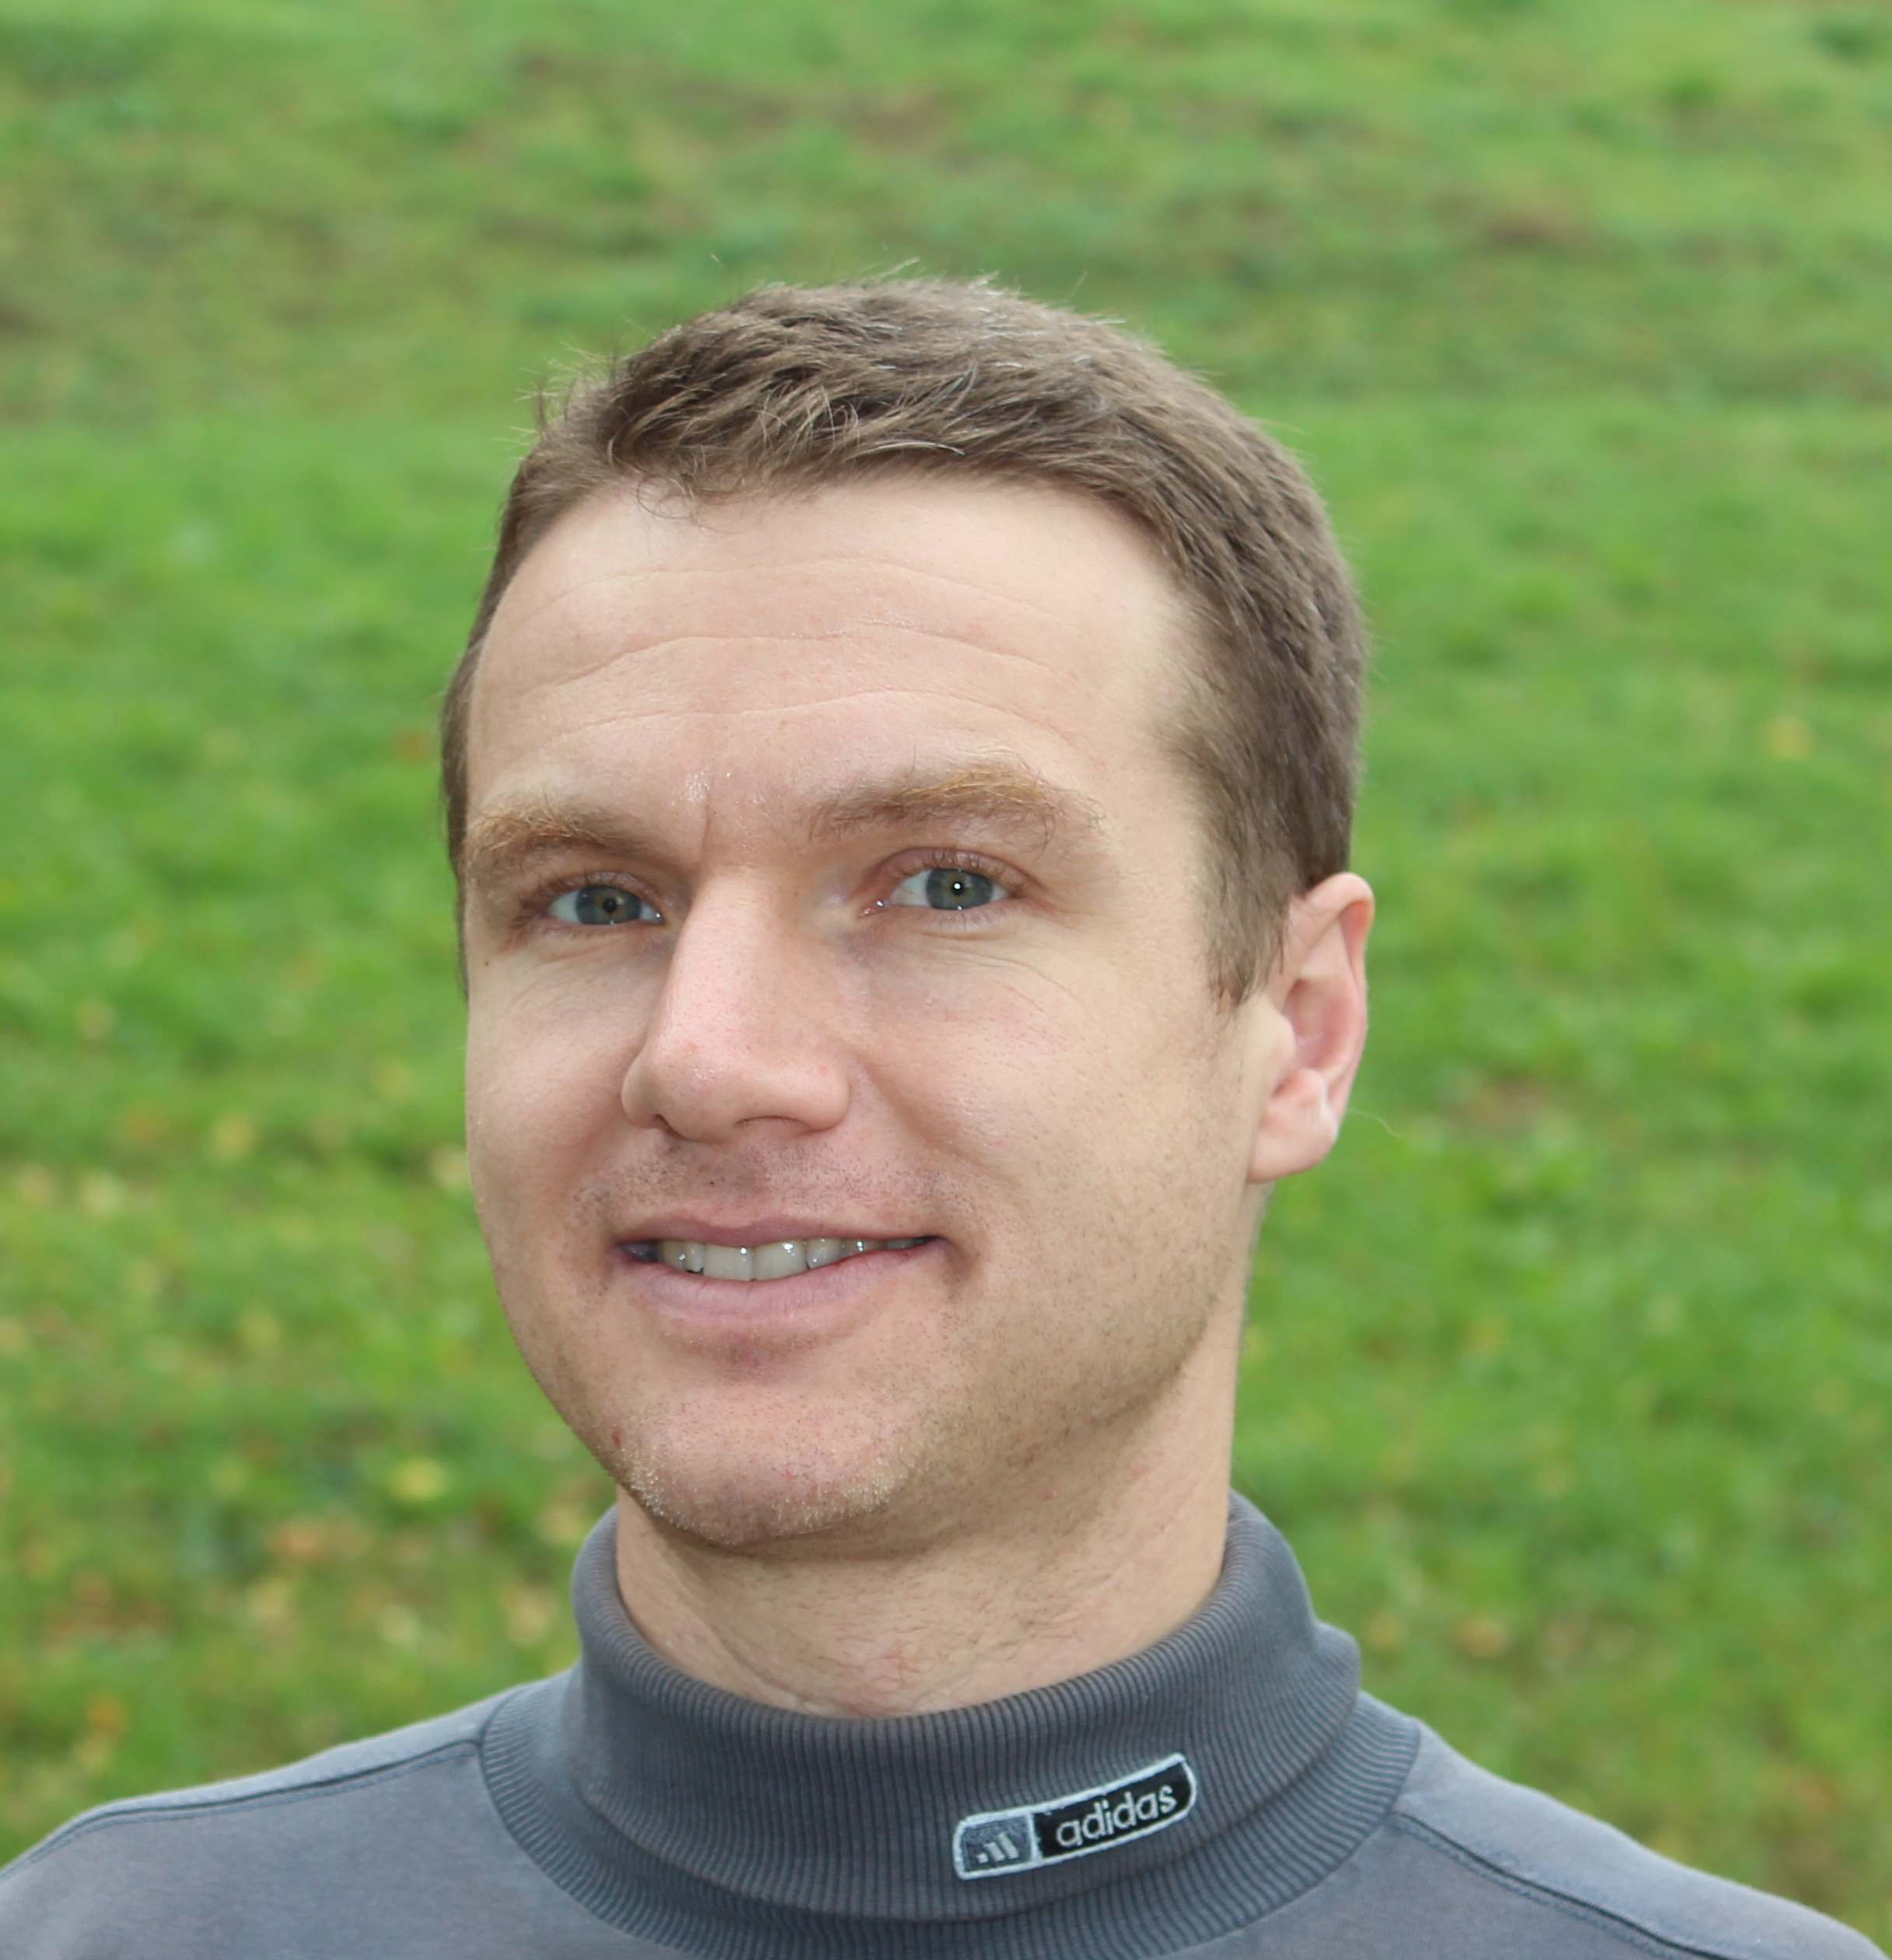
\includegraphics[height=4cm]{MarkusMueller.jpg}
	\end{minipage}
	\begin{minipage}[c]{10cm}
	Markus Müller
	\end{minipage}
	\begin{minipage}[c]{5cm}
	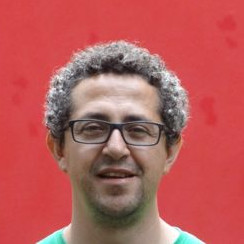
\includegraphics[height=4cm]{Sierra.jpg}
	\end{minipage}
	\begin{minipage}[c]{10cm}
	Carlos Sierra
	\end{minipage}
	\begin{minipage}[c]{5cm}
	
\includegraphics[height=4cm]{qrcode.png}
	\end{minipage}
     \end{minipage}
\vspace{1cm}
}

\usepackage{setspace}
\setstretch{1.25}

\usepackage{bm}
\usepackage{tikz}
\usetikzlibrary{arrows,backgrounds,calc,chains,fadings,fit,graphs,mindmap,patterns,positioning,quotes,scopes,shapes.geometric,trees} 

\definecolor{yellow}{rgb}{1,1,0}
\definecolor{green}{rgb}{0,1,0}
\definecolor{GeneralModel}{rgb}{0.709803921568627,0.870588235294118,0.63921568627451}
\definecolor{TheoreticalAnalysis}{rgb}{1,1,0.8}
\definecolor{SoilPy}{rgb}{0.63921568627451,0.83921568627451,0.8}
\definecolor{SoilR}{rgb}{0.8,0.8,1}

\colorlet{lightblue}{blue!25}
\colorlet{darkblue}{blue!75}
\colorlet{lightpink}{red!12}
\colorlet{darkred}{red!75}
\colorlet{red}{red!50}
\colorlet{LTICTBg}{lightpink}
\colorlet{GASDSTBg}{blue}
\colorlet{LDSTBg}{yellow!30!blue!30}

%%%%<
%\usepackage{verbatim}
%\usepackage[active,tightpage]{preview}
%\PreviewEnvironment{tikzpicture}
%\setlength\PreviewBorder{5pt}%
%%%%>

%node[pos=0.5]{yes}
\DeclareRobustCommand{\intl}{\int\limits}
\newcommand{\tens}[1]{\mathbf{\mathrm{#1}}}
\renewcommand{\vec}[1]{\mathbf{#1}}
\newcommand{\deriv}[1]{\frac{d}{d#1}}

\pgfkeys{/TNIoft/.code={$\mathbf{I}(t)$, $\mathbf{N}(t)$, $\mathbf{T}(t)$?}}
\pgfkeys{/fofC/.code={$\TM(\CM)$,$\NM(\CM)$ ?}} 
\pgfkeys{/foft/.code={$\TM(t),\NM(t)$?}} 
\pgfkeys{/ipsi/.code={$\IM(t)=\xi(t)\IM$?}} %the extra { } are needed to escape =
\pgfkeys{/iper/.code={$\IM(t)$ periodic?}}
\pgfkeys{/iconst/.code={$\IM(t)$ const.?}}
\pgfkeys{/stab/.code={S}}

\tikzset{
  every node/.style={font=\sfs},%,text depth=.2ex},
  test/.style={diamond,draw,minimum width=.5em,text width=2em,aspect=1,align=center  },
  comment/.style={rectangle,text width=3cm,minimum width=1cm,align=center},
  decision/.style = {test}, 
  sact/.style    = { rectangle, draw=blue, thick, 
                        fill=blue!20, text width=9em, 
                        rounded corners, minimum height=1cm},
  description/.style    = { rectangle, draw=black, thick, 
                        fill=black!20, text width=12em, text centered,
                        rounded corners, minimum height=.5em},
  ce/.style    = { circle, draw=black, thick, 
                        fill=blue!20, text width=1em, text centered,
                        rounded corners, minimum height=1em},
  cst/.style={draw, black, circle,text width=1em,child anchor=south},
  cex/.style={draw=black,fill=white, circle,text width=1em,minimum height=1em,align=center,text=red,node font=\bf},
  ceok/.style={draw=black,fill=white, circle,text width=1em,minimum height=1em,align=center,text=green,node font=\bf},
  line/.style     = { draw, thick, ->, shorten >=2pt }
}

%\setbeamersize{text margin left=5pt,text margin right=5pt}
%\newtheorem{theorem}{Theorem} 
\newtheorem{Def}{Definition:}
%\newtheorem{lemma}{Lemma:}

%%%%%%%%%%%%%%%%%%%%%%%%%%%%%%%%%%%%%%%%%%%%%%%%%%%%%%%%%%%%%%%%%%%%%%%%%%%%%%%%%%%%%%
\begin{document}
\graphicspath{ {./images/} }
\begin{frame}
%	\begin{center}
%\input{uas.tex}
%	\end{center}
\begin{columns}
  % ------------
  % FIRST COLUMN
  % ------------
  
  \begin{column}{.48\textwidth}
    \begin{minipage}[T]{.95\textwidth}
      %%%%%%%%%%%%%%%%%%%%%%%%%%%%%%%%%%%%%%%%%%%%%%%%%%%%%%%%%%%%%%%%%%%%%%%%%%%%%%%%%%%%%%
      \setbeamercolor*{block title}{bg=darkgray}
      \begin{block}{Overview}
	\begin{figure}
	  \includegraphics[height=20cm]{soilrMindMap.pdf}
	  \caption{The General Model concept as central synthesis tool and product of theory and software development}
	\end{figure}
      \end{block}
    %%%%%%%%%%%%%%%%%%%%%%%%%%%%%%%%%%%%%%%%%%%%%%%%%%%%%%%%%%%%%%%%%%%%%%%%%%%%%%%%%%%%%%
    \setbeamercolor*{block title}{bg=GeneralModel}
    \begin{block}{The General SOM Decomposition Model}
    \begin{columns}[b]
    \column{.5\textwidth}
    		\[
		\mathbf{\dot{C}}= \bm{I}(t) + {\bf T}(\mathbf{C},t) \cdot {\bf N}(t, \bm{C}) \cdot \bm{C}(t)
    		\]
    		\begin{equation*}	
    		\label{structCond}
    		\begin{array}{lcl}	
    		N_{i,i}(\mathbf{C},t) 		&\ge& 	 0 \quad \forall i \\
    		T_{i,i}(\mathbf{C},t) 		&=& 	 -1 \quad \forall i \\
    		T_{i,j}(\mathbf{C},t) 		&\ge& 	 0 \quad \forall i \ne j \\
    		\sum_i T_{i,j}(\mathbf{C},t) 	&=  &	 1\quad \forall j 
    		\end{array}	
    		\end{equation*}	
    		This model structure generalizes most SOM decomposition models with any arbitrary number of pools, including those describing nonlinear interactions among state variables. It enforces mass balance and substrate dependence of decomposition, and it is fexible enough to describe:
		\begin{enumerate}
		\item Heterogeneity of decomposition rates
		\item Transformations of organic matter
		\item Environmental variability effects
		\item Organic matter interactions
		\end{enumerate}

    \column{.5\textwidth}
		Examples for nonlinear models are:
		\begin{enumerate}
			\item Exoenzyme models \citep{Schimel,Sinsabaugh}
			\item AWB \citep{Allison}
			\item Bacwave \citep{Zelenev}
			\item MEND \citep{WangMEND}
			\item Manzoni \citep{Manzoni07}
		\end{enumerate}
		Also linear models fit into the general framework 
		\begin{enumerate}
			\item Henin's model \citep{HeninDupuis, Henin}
			\item ICBM \citep{AndrenKatterer}
			\item RothC \citep{Jenkinson, Coleman} 
			\item Century \citep{Parton} 
			\item Fontaine 1-4 \citep{Fontaine}
		\end{enumerate}
    \end{columns}
    \end{block}
      %%%%%%%%%%%%%%%%%%%%%%%%%%%%%%%%%%%%%%%%%%%%%%%%%%%%%%%%%%%%%%%%%%%%%%%%%%%%%%%%%%%%%%
      \setbeamercolor*{block title}{bg=SoilPy}
      \begin{block}{
	  \includegraphics[height=1.5cm]{logo_soilpy} 
	  \hspace{1cm}
	  python Software, not yet published 
	  }
	\begin{enumerate}
		\item A dynamic  catalog to \emph{reproduce} the symbolic math representations of all the above 
		mentioned models in terms of the general model structure.
		\item Tools to check the validity of the models (properties of $\mathbf{T}$ and $\mathbf{N}$)
		\item Tools to verify symbolically available fixed points 
		\item Tools to analyze the stability of those fixed points
		\item Tools to compute and verify fixed points numerically
		\item Tools to visualize 2-pool and 3-pool models in the phase space 
		\item Symbolic coordinate transformations to facilitate stability analysis
	\end{enumerate}
The following example \citep{Manzoni07} is copied from the (shortened) \LaTeX \hspace{1ex}  report of the software:\\ 
$\frac{d}{d{t}}\left(\begin{matrix}C_{S}\\C_{B}\end{matrix}\right)=\left(\begin{matrix}ADD - \frac{C_{B} C_{S} k_{S}}{C_{S} + K_{m}} + C_{B} k_{B}\\\frac{C_{B} C_{S} k_{S}}{C_{S} + K_{m}} \left(- r + 1\right) - C_{B} k_{B}\end{matrix}\right) $
translates to 
$ \mathbf{\dot{C}}=\mathbf{I + T\cdot N(C)\, C} $\\
with: $\mathbf{\dot{C}}=\frac{d}{d{t}}\left(\begin{matrix}C_{S}\\C_{B}\end{matrix}\right)$,
$\mathbf{T}=\left(\begin{matrix}-1&  1\\- r + 1 & -1\end{matrix}\right)$,
$\mathbf{N}=\left(\begin{matrix}\frac{C_{B} k_{S}}{C_{S} + K_{m}} & 0\\0 & k_{B}\end{matrix}\right) \text{}$,
$\mathbf{I}=\left(\begin{matrix}ADD\\0\end{matrix}\right)$.\\ 
Checking alphas:
$ r_{0}=-\sum_{k=1}^{n}T_{k,0}=r $ ,$ r_{1}=-\sum_{k=1}^{n}T_{k,1}=0 $.\\
Checking suggested symbolic fixed point(s):
$ \mathbf{\tilde{C}}=\left(\begin{matrix}\frac{K_{m} k_{B}}{- k_{B} + k_{S} \left(- r + 1\right)}\\\frac{ADD}{k_{B} r} \left(- r + 1\right)\end{matrix}\right)$, substitute:
$ \mathbf{\dot{C}}(\mathbf{\tilde{C}})=\left(\begin{matrix}0\\0\end{matrix}\right) $\\
With numeric parameters:
$ \mathbf{\dot{C}}=\left(\begin{matrix}- \frac{1.8 \cdot 10^{-5} C_{B} C_{S}}{C_{S} + 900} + 0.007 C_{B} + 3.3\\\frac{7.2 \cdot 10^{-6} C_{B} C_{S}}{C_{S} + 900} - 0.007 C_{B}\end{matrix}\right) $
	\begin{figure}
	  \includegraphics[height=11cm]{posfp.pdf}
	  \includegraphics[height=11cm]{3D-OscillatingStayPositiveExample}
	  \caption{On the left is the phase plane plot of a model with a fixed point. On the left is a phase space plot of a linear 3 pool feedback model showing the plane of damped  oscillations and the boundaries of the positive octant.
	  }
	\end{figure}
      \end{block}
    \end{minipage}
  \end{column}
  
    %%%%%%%%%%%%%%%%%%%%%%%%%%%%%%%%%%%%%%%%%%%%%%%%%%%%%%%%%%%%%%%%%%%%%%%%%%%%%%%%%%%%%%
  % -------------
  % SECOND COLUMN
  % -------------
  
  
  \begin{column}{.48\textwidth}
    \begin{minipage}[T]{.95\textwidth}
      %%%%%%%%%%%%%%%%%%%%%%%%%%%%%%%%%%%%%%%%%%%%%%%%%%%%%%%%%%%%%%%%%%%%%%%%%%%%%%%%%%%%%%
      \setbeamercolor*{block title}{bg=TheoreticalAnalysis}
      \begin{block}{Theoretical Stability Analysis}
      The unified description of many models in one formula offers: 
      \begin{enumerate}
	\item 
	A strict and unambiguous definition and  treatment of different concepts, e.g. \emph{Stability}. 
	\item
	Access to existing and relevant mathematical literature by the right keywords. 
	\item 
	Means to classify models w.r.t. mathematical properties and thereby:
	\item 
	A way to decide which questions to ask about which models, thereby providing both of the following: 
	\item 
	Inspiration for generalization, a focal point to answer many questions about many models at once, or
	\item 
	Protection against futile quests by discovering unanswerable questions, e.g. \emph{steady} states for time\emph{variant} systems... 
      \end{enumerate}
	\begin{figure}
	\newlength{\ab}
\setlength{\ab}{3em}
\newlength{\lsdone}
\newlength{\ldone}
\newlength{\lsdtwo}
\newlength{\lsdthree}
\newlength{\lsdfour}
\setlength{\lsdone}{.9\textwidth}
\setlength{\ldone}{.13\lsdone}
\setlength{\lsdtwo}{    .5\lsdone}
\setlength{\lsdthree}{ .25\lsdone}
\setlength{\lsdfour}{ .125\lsdone}
\newlength{\radius}
\setlength{\radius}{.5\textwidth}
\newlength{\subwidthlr}
\setlength{\subwidthlr}{.45\textwidth}

	    \begin{tikzpicture}
  [ 
    %mindmap,
    every node/.style={fill=white,execute at begin node=\hskip0pt,font=\tiny},
    level 1/.append style={level distance=\ldone,sibling distance=\lsdone},
    level 2/.append style={sibling distance=\lsdtwo},
    level 3/.append style={sibling distance=\lsdthree},
    level 4/.append style={sibling distance=\lsdfour},align=center
  ]
  \node[cst](cst) {root}
  %\pgfpathcircle{\pgfpointanchor{x}{north}}{2pt}
    child{
      node[test](TNIoft) {\pgfkeys{/TNIoft}} 
      %child[concept color=red]{
      %    node[proc] {BiBo, CiCo or ISS } 
          child{
            node[test](CLorNL){\pgfkeys{/fofC}}
            edge from parent[parent anchor=west,child anchor=north, edge from parent path={\mypath}]
                child{
                  node[test](NLTIorNLTV){\pgfkeys{/foft}}
                  child{
                    node[test]{tv ISS proof}
                    child{
                      node[ce](mark){}
                      edge from parent[parent anchor=west,child anchor=north, edge from parent path={\mypath}]
	    	    } 
		    child[missing]{}
                    edge from parent[parent anchor=west,child anchor=north, edge from parent path={\mypath}]
	    	  } 
                  child{
                    node[test]{ISS proof}
                    child{
                      node[ce] {}
                      edge from parent[parent anchor=west,child anchor=north, edge from parent path={\mypath}]
	    	    } 
		    child[missing]{}
                    edge from parent[parent anchor=east,child anchor=north, edge from parent path={\mypath}]
	    	  } 
                    edge from parent[parent anchor=west, edge from parent path={\mypath}]
		}
              child{
                node[test](LTIorLTV) {\pgfkeys{/foft}} 
                child{
                  node[test](LTV){UAS proof}
                  child{
                    node[ce]{}
                    edge from parent[parent anchor=west,child anchor=north, edge from parent path={\mypath}]
	    	  } 
		  child[missing]{}
                  edge from parent[parent anchor=west,child anchor=north, edge from parent path={\mypath}]
	    	} 
                child{
                  node[ce](LTI){}
                  edge from parent[parent anchor=east,child anchor=north, edge from parent path={\mypath}]
	    	} 
                edge from parent[parent anchor=east,edge from parent path={\mypath}]
              }
	  node[left,fill=none]{yes}
	  }
	  %%%%%%%%%%%%%%%%%%%%%%%%%%%%%%%%%%%%%%%%%%%%%%%%%%%%%%%%%
          child{
            node[test](DLorNL){\pgfkeys{/fofC}}
              child{
                  node[test](GAS){GAS proof}
                  child{
                    node[ce]{}
                    edge from parent[parent anchor=west,child anchor=north, edge from parent path={\mypath}]
	    	  } 
                  child{
                    node[test]{AS proof per FP}
                    child{
                      node[ce](ASend) {}
                      edge from parent[parent anchor=west,child anchor=north, edge from parent path={\mypath}]
	    	    } 
		    child[missing]{}
                    edge from parent[parent anchor=east,child anchor=north, edge from parent path={\mypath}]
	    	  } 
                    edge from parent[parent anchor=west, edge from parent path={\mypath}]
		}
              child{
                node[ce](LTC) {} 
                edge from parent[parent anchor=east,edge from parent path={\mypath}]
              }
            edge from parent[parent anchor=east,child anchor=north, edge from parent path={\mypath}]
	    node[above,fill=none]{no}
	  }
    };
  %\begin{scope}[every annotation/.style={fill=black!40}]
  %	\node [annotation, above] at (CLorNL.north east) {
  %	{Control Theory}
  %};
  %\end{scope}
  \begin{pgfonlayer}{background}
    %\clip (-1.5,-5) rectangle ++(4,10);
    % The large rectangles:
    % first find the coordinates of the boundaries
    
    \fill [pink] (cst) rectangle (mark);
    \fill [lightblue] let \p1=(mark),\p2=(mark) in
    	(cst) rectangle (-\x1,\y2); 
    % level 2rectangles:
    \fill [red] (CLorNL) rectangle (mark);
    \fill[blue] let \p1=(cst),\p2=(mark) in  
    	(DLorNL) rectangle(\x1,\y2);
    % level 3rectangles:
    \fill[lightpink] let \p1=(cst),\p2=(mark) in  
    	(LTIorLTV) rectangle (\x1,\y2);
    \fill [darkred] (NLTIorNLTV) rectangle (mark);
    \fill [darkblue] let \p1=(DLorNL),\p2=(GAS) in
    	(ASend) rectangle (\x1,\y2); 
    
    \path(CLorNL) node[draw=pink,rectangle,fill=none,above=\ab]{\hfs Control Theory};
    \path(NLTIorNLTV) node[draw=none,rectangle,fill=none,above=\ab]{\hfs nonlinear};
    \path(LTIorLTV) node[draw=none,rectangle,fill=none,above=\ab]{\hfs linear};
    
    \path(GAS) node[draw=none,rectangle,fill=none,above=\ab]{\hfs nonlinear};
    \path(LTC) node[draw=none,rectangle,fill=none,above=\ab]{\hfs linear};
    
    \path(LTV) node[draw=none,rectangle,fill=none,above=\ab]{\hfs LTV};
    \path(LTI) node[draw=none,rectangle,fill=none,above=\ab]{\hfs LTI};
    \path(DLorNL) node[draw=lightblue,rectangle,fill=none,above=\ab, text width=.2\lsdone]{\hfs Dynamic System Theory};
  \end{pgfonlayer}
\end{tikzpicture} 

	  \caption{The graph shows one example about how the general model can guide decisions. Given an arbitrary instance of the general model, it  shows which  mathematically defined concept of \emph{stability} can possibly be established based on the mathematical properties of the model.}
	\end{figure}
      \end{block}
      %%%%%%%%%%%%%%%%%%%%%%%%%%%%%%%%%%%%%%%%%%%%%%%%%%%%%%%%%%%%%%%%%%%%%%%%%%%%%%%%%%%%%%
      \setbeamercolor*{block title}{bg=SoilR}
      \begin{block}{
	  \includegraphics[height=1.5cm]{logo_soilr} 
	  \hspace{1cm}
	  R Software,
	  public package on cran
	  }
	 SoilR is our publicly available code representation of the general model. It consists of both an extensive library of models and many computational tools to analyze them.  Its internal representation as object oriented framework helped the present form of the general model to emerge. In particular its purposes are the following:
	 \begin{enumerate}
	 \item Prove theoretical concepts by implementing them, exposing theoretical errors and ambiguities by the rigor required to run the code.
	 \item Disclose the underlying theoretical structure of the ecological system by the continuous restructuring required to integrate new non-contradictory features
	 \item Provide an easy to use framework to reproduce our scientific results
	 \item Provide a community tool that can be improved and modified by others, facilitating \emph{reproducible research}. 
	 \end{enumerate}
	 

	\begin{figure}
	  \includegraphics[height=9cm]{RothCfig} \hspace{1cm}
	  \includegraphics[height=9cm]{ModelFit.pdf}
	  \includegraphics[height=9cm]{NonlinearAtmosphericModelMeanAge}
	  %\includegraphics[height=10cm]{NonlinearAtmosphericModelMeanAge}
	  %\includegraphics[height=10cm]{MeanAgeSteady}
	  %\includegraphics[width=.3\textwidth]{CDI}
	  %\includegraphics[width=.5\textwidth]{PoolStructureEx.pdf}
	  \caption{
	  %\begin{minipage}{\textwidth}
	  Example applications of SoilR, 
	  left: carbon stocks, total and per pool, predicted by the Roth C model as functions of time; 
	   middle: example of a Bayesian parameter estimation combining SoilR with package FME.   
	   right: Mean age of carbon in a pool of an nonlinear model as function of time.
	  %\end{minipage}
	  }
	\end{figure}
	\begin{figure}
	  \includegraphics[height=7cm]{Reservoir_Peoples_Ages2}
	  \includegraphics[height=7cm]{MeanTransitTime}
	  %\includegraphics[width=.45\textwidth]{Reservoir_Peoples_Ages2}
	  %\includegraphics[width=.45\textwidth]{MeanTransitTime}
	  %\includegraphics[width=.45\textwidth]{NonlinearAtmosphericModelMeanAge}
	  %\includegraphics[width=.45\textwidth]{MeanAgeSteady}
	  \caption{Two intuitive definitions of mean age and transit time, implemented in SoilR for non-steady-state models. }
	\end{figure}
	We are currently developing a new method for calculating transit times and mean ages for models that are not in equilibrium and can also be nonlinear. 
	This is done with a Monte Carlo particle simulator that facilitates modeling of cycling times through a network of compartments. All particles in the system
	contain information about the time they enter the system, how long they have remained, and how old they are at the time they leave the system. 

      \end{block}

    \end{minipage}
  \end{column}
\end{columns}
	\vspace{3ex}
\end{frame}
\bibliography{GeneralModel}
\bibliographystyle{abbrvnat}
\end{document}
